\chapter{Procedimiento de la Construcción}
% licitaciones -> Precios unitarios
% Empresas privadas
% Consultorías
% Evaluaciones estatales
% Diplomado

% Trabajo final 15%
% Curso en línea 1 semana
% Aditec
% Ecosoft
% Zamora

% Horario de asesorías
% Se va a las 3
% Hay una relación entre la ingeniería, irrigación y la construcción
% Ensayo - Primera participación a mano, saber redactar 1 cuartilla, poder consultar bibliografía, presa del cajón
% Martes 29
% Puente baluarte 

\section{Introducción}
\begin{definition}[Construcción]
    Es una palabra originaria del latón con componentes léxicos como el prefijo ``con'' que quiere decir completamente o globalmente y ``estruere'' que significa juntar o amontonar, más el sufijo ``cion'' que es acción y efecto.

    También hacer referencia al conjunto de personas y materiales que tienen relación con la fabricación de edificios, obras arquitectónicas o de ingeniería. Este vocablo se le otorga a la rama de la arquitectura y la ingeniería civil, y son los proyectos de construcción y efectuación de la infraestructura con diferentes procesos, entre ellos el presupuestado, planificación de objetivos en el tiempo, seguridad, recursos humanos, logística, etc.
\end{definition}
% ¿Por qué construir? Venciendo el reto de la sierra madre occidental, carretera durango-mazatlan
% Multianuales
Los servicios relacionados con la obra pública son: el Anteproyecto, Proyecto ó Diseño, y la construcción es la parte de la obra pública
% Por la necesidad de abastecer agua para regar en más área frente al incremento de parcelas agrícolas tecnificadas.
\begin{itemize}
    \item Estudios y proyectos
    \item Proyecto ejecutivo: Si una empresa hace los estudios y proyectos no puede construirlas
    \item Planeación la hace la institución involucrada
    \item Construcción: Si una empresa construye, no puede supervisarla
    \item Supervisión
\end{itemize}
Exceptuando, los proyectos integrales (llave en mano) se puede proyectar y construir
% En primer estancia está la ley, LOP y SRM
% Reglamento: RCOP y SRM 
% Manuales
% Lineamientos
% Normas
En México, la ley indica que se tiene que hacer una serie de estudios y proyectos para aprobar la obra, por lo tanto se construye y supervisa.

La supervisión es un estudio relacionado con la construcción, con la cual la ley queda clara, si la empresa que la construye no puede supervisarla.
% Vicios ocultos

¿Cuáles son los proyectos y estudios para hacer una Zona de Riego?
\begin{itemize}
    \item Levantamiento topográfico: Estudio topográfico
    \item Estudio Agrológico: Incluye la parte de precipitación, temperatura, suelo
    \item Proyecto Ejecutivo de la zona de riego: Integración del expediente
    \item Estudio Socioeconómico: Antecedentes históricos sobre qué cultivos se habían sembrado en ese lugar
    \item Manifestación de impacto ambiental
\end{itemize}
\textbf{Planeación de obra}: Como un nexo entre el proyecto ejecutivo y la construcción

Caminos de acceso, desarraigo, construcción de nuevas ciudades o localidades, todo esto se considera dentro del costo.

La relación de la irrigación en la construcción: Formar profesionales competentes en el campo de la irrigación y aprovechamientos hídricos, para contribuir a su evaluación, conservación, uso y manejo, tratamiento y reutilización bajo un enfoque integral y sostenible, con fines principalmente agropecuarios; mediante la planeación, realización de estudios y proyectos, construcción, operación, mantenimiento y rehabilitación de la infraestructura hidráulica para coadyuvar en la producción agroalimentaria del país y a su desarrollo económico y social.

Proceso de contratación:
\begin{itemize}
    \item Planeación
    \item Procedimientos de contratación
    \item Procedimientos concluidos
    \item Contratos
    \item Ejecución
\end{itemize}
\begin{definition}[Procedimiento]
    Es la acción de proceder, forma de ejecutar las cosas; poner en ejecución, que en algunos casos se puede confundir con proceso
\end{definition}
\begin{definition}[Proceso]
    Es el conjunto de las fases sucesivas
\end{definition}
\section{Especificaciones de la Construcción.}
Espinobarros (1988) es el camino forma o sistema para llevar a cabo una obra de ingeniería. Con la finalidad de satisfacer una necesidad humana, a través de la aplicación de la experiencia, el conocimiento y el ingenio que el hombre posee.

Mendoza dice que el Procedimiento Constructivo son las actividades lógicas que permitirán el uso de los recursos disponibles en cantidad y calidad tales que la obra sea de la mejor calidad posible y se efectúa a un costo razonable y en el tiempo previsto.

Olguín refiere que un procedimiento constructivo son las actividades que en forma secuencial y en base a un programa de trabajo, permitirán ejecutar un proyecto en el tiempo y con los costos adecuados, para lograr su materialización de manera que se tenga una obra con calidad y economía

El procedimiento de la construcción debe estudiar las actividades en forma secuencial, los aspectos relevantes de una obra, para determinar el costo y la duración de la misma (tiempo), y si es posible reducir estos parámetros sin afectar indebidamente el servicio que va a prestar el proyecto en ejecución.

\subsection{Artículo 2.- De la LOPySRM:}
\begin{itemize}
    \item VI. Contratista: la persona que celebre contratos de obras públicas o de servicios relacionados con las mismas; Fracción reformada DOF 28-05-2009
    \item VII. Licitante: la persona que participe en cualquier procedimiento de licitación pública, o bien de invitación a cuando menos tres personas; Fracción reformada DOF 28-05-2009
    \item VIII. Obras públicas asociadas a proyectos de infraestructura: las obras que tienen por objeto la construcción, ampliación o modificación de bienes inmuebles destinados directamente a la prestación de servicios de comunicaciones, transportes, hidráulico, medio ambiente, turístico, educación, salud y energético; Fracción adicionada DOF 28-05-2009
    \item IX. Proyecto ejecutivo: el conjunto de planos y documentos que conforman los proyectos arquitectónico y de ingeniería de una obra, el catálogo de conceptos, así como las descripciones e información suficientes para que ésta se pueda llevar a cabo; Fracción adicionada DOF 28-05-2009
    \item X. Proyecto arquitectónico: el que define la forma, estilo, distribución y el diseño funcional de una obra. Se expresará por medio de planos, maquetas, perspectivas, dibujos artísticos, entre otros; Fracción adicionada DOF 28-05-2009
    \item XI. Proyecto de ingeniería: el que comprende los planos constructivos, memorias de cálculo y descriptivas, especificaciones generales y particulares aplicables, así como plantas, alzados, secciones y detalle, que permitan llevar a cabo una obra civil, eléctrica, mecánica o de cualquier otra especialidad, y Fracción adicionada DOF 28-05-2009
\end{itemize}
\begin{definition}[Concepto de obra]
    Descripción de la actividad que se va a realizar con base en las especificaciones, normas de calidad y de acuerdo a lo que marque el contratista
\end{definition}

El concepto es el análisis de agua con fines potables y esta obliga cumplir con una norma de la Secretaría de Salud.

\textbf{Artículo 3}. Para los efectos de esta Ley, se consideran obras públicas los trabajos que tengan por objeto construir, instalar, ampliar, adecuar, remodelar, restaurar, conservar, mantener, modificar y demoler bienes inmuebles. Asimismo, quedan comprendidos dentro de las obras públicas los siguientes conceptos:
\begin{itemize}
    \item I El mantenimiento y la restauración de bienes muebles incorporados o adheridos a un inmueble, cuando implique modificación al propio inmueble;
    \item III Los proyectos integrales, en los cuales el contratista se obliga desde el diseño de la obra hasta su terminación total, incluyéndose, cuando se requiera, la transferencia de tecnología;
    \item IV Los trabajos de exploración, localización y perforación distintos a los de extracción de petróleo y gas; mejoramiento del suelo y subsuelo; desmontes; extracción y aquellos similares, que tengan por objeto la explotación y desarrollo de los recursos naturales que se encuentren en el suelo o en el subsuelo;
    \item VI. Los trabajos de infraestructura agropecuaria;
    \item VII. La instalación, montaje, colocación o aplicación, incluyendo las pruebas de operación de bienes muebles que deban incorporarse, adherirse o destinarse a un inmueble, siempre y cuando dichos bienes sean proporcionados por la convocante al contratista; o bien, cuando incluyan la adquisición y su precio sea menor al de los trabajos que se contraten;
    \item VIII. Las asociadas a proyectos de infraestructura que impliquen inversión a largo plazo y amortización programada en los términos de esta Ley, en las cuales el contratista se obligue desde la ejecución de la obra, su puesta en marcha, mantenimiento y operación de la misma, y
\end{itemize}

\textbf{Artículo 2}. Del Reglamento de la LOPySRM se aplicarán las definiciones establecidas en el artículo 2 de la Ley. Asimismo, se entenderá por:
\begin{itemize}
    \item XI. Especificaciones generales de construcción: el conjunto de condiciones generales que las dependencias y entidades tienen establecidas para la ejecución de obras, incluyendo las que deben aplicarse para la realización de estudios, proyectos, ejecución, equipamiento, puesta en servicio, mantenimiento y supervisión, que comprenden la forma de medición y la base de pago de los conceptos de trabajo;
    \item XII. Especificaciones particulares de construcción: el conjunto de requisitos exigidos por las dependencias y entidades para la realización de cada obra, mismas que modifican, adicionan o sustituyen a las especificaciones generales de construcción;
    \item VIII. Bitácora: el instrumento técnico que constituye el medio de comunicación entre las partes que formalizan los contratos, en el cual se registran los asuntos y eventos importantes que se presenten durante la ejecución de los trabajos, ya sea a través de medios remotos de comunicación electrónica, caso en el cual se denominará Bitácora electrónica, u otros medios autorizados en los términos de este Reglamento, en cuyo caso se denominará Bitácora convencional;
    \item XIV. Estimación: la valuación de los trabajos ejecutados en un periodo determinado presentada para autorización de pago, en la cual se aplican los precios, valores o porcentajes establecidos en el contrato en atención a la naturaleza y características del mismo, considerando, en su caso, la amortización de los anticipos, los ajustes de costos, las retenciones económicas, las penas convencionales y las deducciones; así como, la valuación de los conceptos que permitan determinar el monto de los gastos no recuperables;
    \item XXIX. Superintendente: el representante del contratista ante la dependencia o la entidad para cumplir con los términos y condiciones pactados en el contrato, en lo relacionado con la ejecución de los trabajos.
\end{itemize}

\begin{definition}[Liquidación]
    Valorización del importe de las obras ejecutadas y estimadas
\end{definition}
\begin{definition}[Plazo de entrega]
    El lapso de que dispone el contratista para la ejecución de una obra a satisfacción de la institución. Los días, meses o años que se utilicen para determinar en dicho lapso se entenderán naturales del calendario.
\end{definition}
\begin{definition}[Precios unitarios]
    Remuneración al contratista por obra que ejecute en cada concepto y que comprende el pago de todas las erogaciones que haya efectuado el contratista para la ejecución del mismo, de acuerdo con las especificaciones, así como su utilidad y los intereses del capital invertido.
\end{definition}
\begin{definition}[Concepto de trabajo]
    Es la descripción de cada uno de los trabajos que deben integrar una obra.
\end{definition}
\begin{definition}[Catálogo de conceptos]
    Es la relación de los diversos conceptos de trabajo que intervienen en la ejecución de las obras.
\end{definition}
\begin{definition}[Programa de trabajo]
    Documento que muestra las cantidades de obra que deberá realizar el contratista en cada uno de los conceptos del catalogo y en cada uno de los meses que comprenda el plazo de entrega de la obra.
\end{definition}
\begin{definition}[Proyecto]
    Conjunto de planos, datos, normas especificaciones, etc. A los que debe ajustarse la ejecución de una obra.
\end{definition}
\begin{definition}[Subcontratista]
    Persona, firma o corporación que mediante autorización previa de la institución y del fiador del contratista, se hace cargo de la ejecución de la obra contratado o de alguna parte de ella, conforme a un contrato que a su vez celebra con el contratista.
\end{definition}
\begin{definition}[Banco de préstamo]
    Sitio aprobado por la institución contratante para la extracción de materiales naturales que sean necesarios para la ejecución de las obras.
\end{definition}
\begin{definition}[Contrato]
    Documento en que se hace constar las, obligaciones y derechos de la institución contratante y el contratista para la realización de una obra u obras determinadas.
\end{definition}
\begin{figure}[h!]
    \centering
      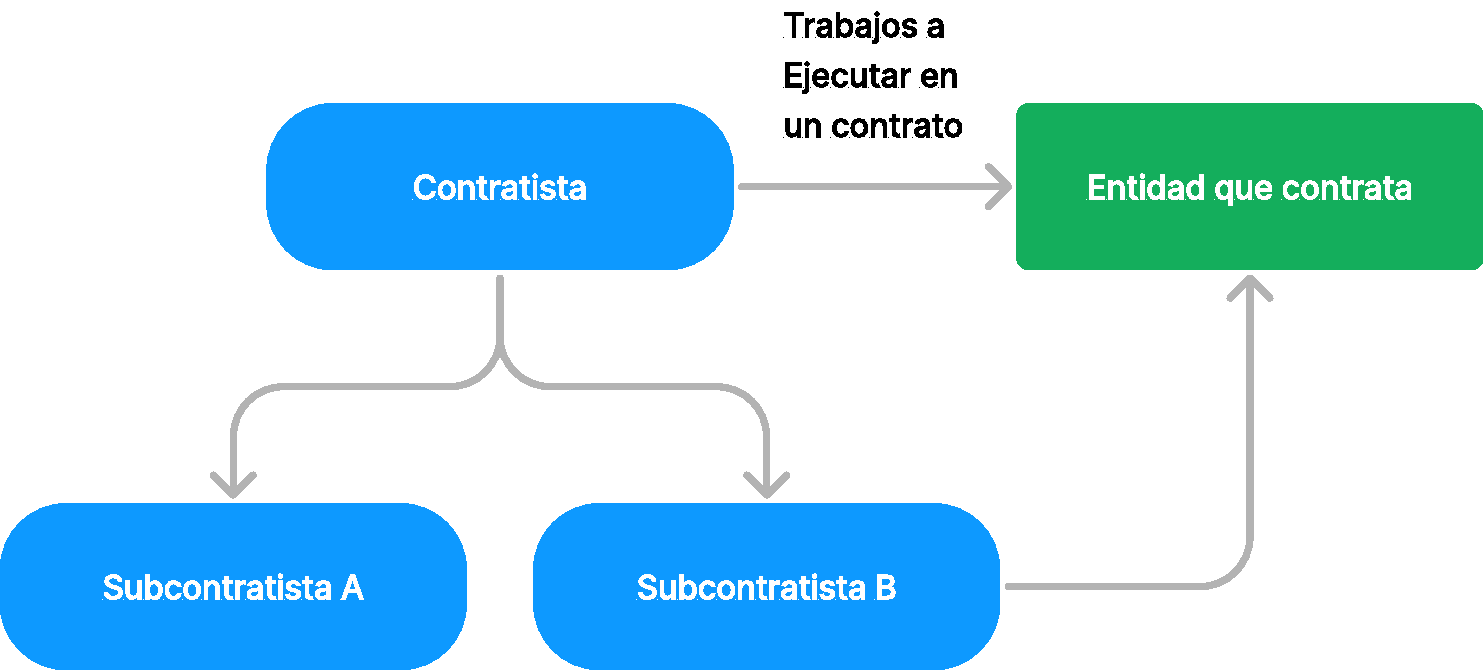
\includegraphics[width=0.5\textwidth]{pc2.pdf}
      \caption{Dinámica del contratista y empresa}
      \label{pc2}
    \end{figure}
\begin{figure}[h!]
\centering
  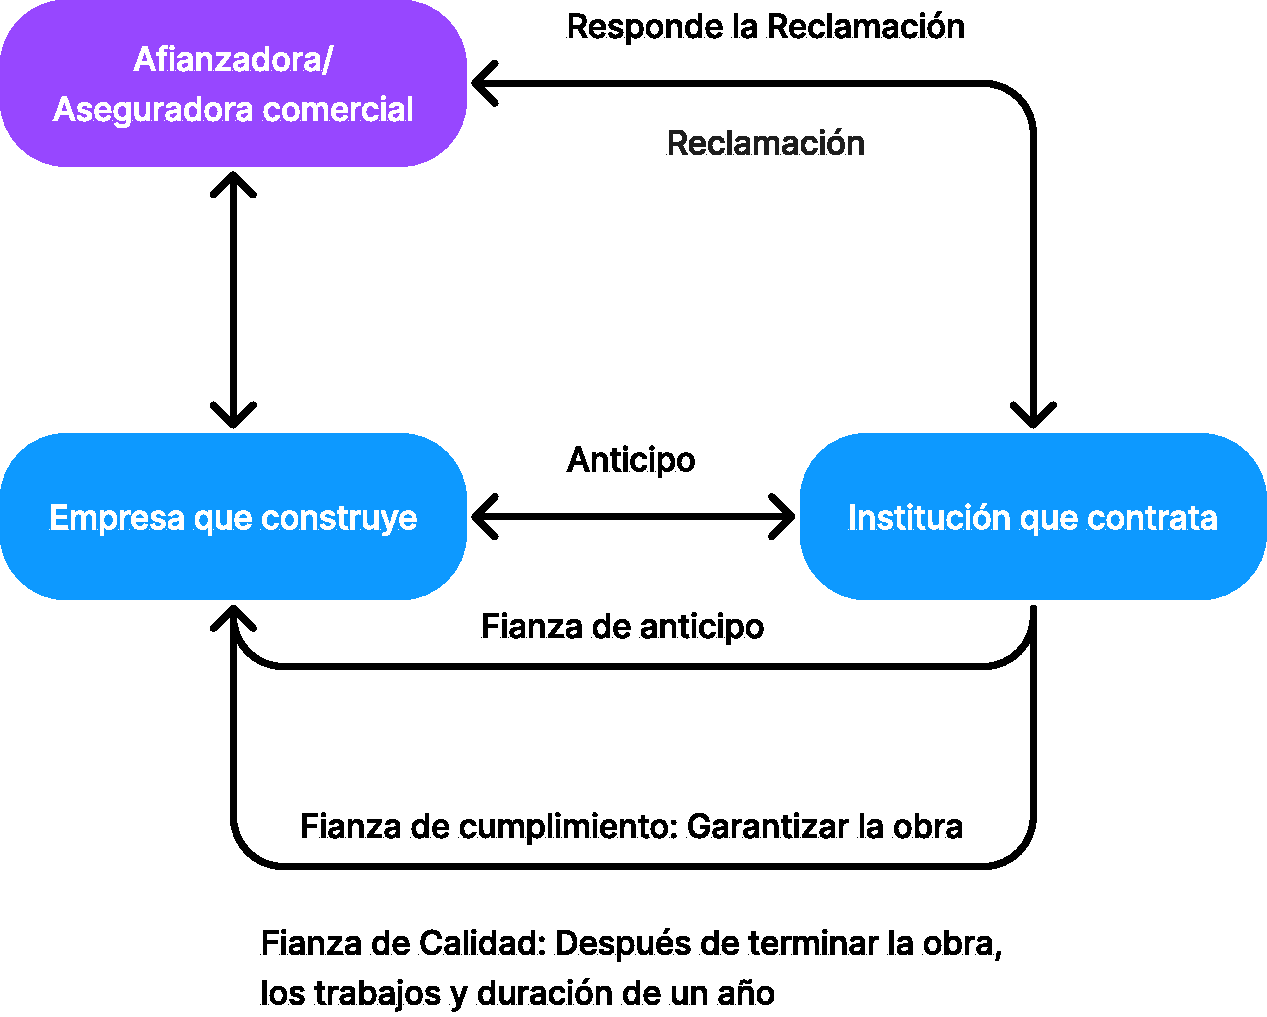
\includegraphics[width=0.5\textwidth]{pc1.pdf}
  \caption{Fianzas. Es una garantía ante un tercero por la responsabilidad de un bien, servicio o efectivo.}
  \label{pc1}
\end{figure}

\begin{itemize}
    \item Garantía de Seriedad: Demostrar que va a cumplir con participar
    \item Garantía por Anticipo: Bueno uso del anticipo
    \item Garantía de Cumplimiento: El contrato se va a cumplir
    \item Garantía de Calidad: Que no haya vicios ocultos
\end{itemize}
% Cámara mexicana de la industria de la construcción
% Abogados en Administración
% https://www.diputados.gob.mx/LeyesBiblio/pdf/56_200521.pdf
Formas de Contratar:
\begin{itemize}
    \item Licitación Pública
    \item Invitación a cuando menos tres personas
    \item Adjudicación Directa
\end{itemize}

Cómo se contratan:
\begin{itemize}
    \item Precios Unitarios
    \item Precio alzado
    \item Mixto
\end{itemize}

\section{Análisis de Precios Unitarios}
Para analizar el precio unitario se tienen que revisar todos los costos involucrados en su ejecución; es decir, en este precio se incluyen los costos directos correspondientes al concepto de trabajo, los costos indirectos, el costo por financiamiento, el cargo por la utilidad del contratista y los cargos adicionales. El análisis, el cálculo y la integración de un precio unitario para un trabajo determinado deben guardar congruencia con los procedimientos constructivos o la metodología de ejecución, con los programas de trabajo y con la utilización de personal, maquinaria y equipo de construcción. Se deben considerar los costos vigentes de los materiales, recursos humanos y demás insumos necesarios en el momento, así como la zona geográfica donde se llevarán a cabo los trabajos, sin impuestos, todo de conformidad con las especificaciones generales y particulares de construcción y las normas de calidad que determine la dependencia o entidad que esté contratando.

\subsection{Costos Directos}
Los costos directos son aquellos que se aplican exclusivamente para la ejecución del concepto, aquí se involucra el material que se utiliza para realizar el concepto, la mano de obra que se requiere y el tiempo utilizado de maquinaría o equipo que interviene en la ejecución del mismo. Para un mejor manejo, se dividen en costos por mano de obra, costos por materiales y costos por equipo y herramientas.

\subsubsection{Costos por mano de obra}
Se deriva de las erogaciones que hace el contratista por el pago de salarios reales al personal que interviene en la ejecución del concepto de trabajo de que se trate, incluyendo al primer mando, entendiéndose como tal hasta la categoría de cabo o jefe de una cuadrilla de trabajadores. No se considerarán dentro de este costo las percepciones del personal técnico, administrativo, de control, supervisión y vigilancia que corresponden a los costos indirectos.

El costo de mano de obra se obtendrá de la expresión:
\begin{equation}
    Mo =\frac{Sr}{R}
\end{equation}
\begin{notation}
    \begin{itemize}
        \item $Mo$ Representa el costo por mano de obra.
        \item $Sr$ Representa el salario real del personal que interviene directamente en la ejecución de cada concepto de trabajo por jornada de ocho horas, salvo las percepciones del personal técnico, administrativo, de control, supervisión y vigilancia que corresponden a los costos indirectos, incluyendo todas las prestaciones derivadas de la Ley Federal del Trabajo, la Ley del Seguro Social, la Ley del Instituto del Fondo Nacional de la Vivienda para los Trabajadores o de los Contratos Colectivos de Trabajo en vigor.
        \item $R$ Representa el rendimiento, es decir, la cantidad de trabajo que desarrolla el personal que interviene directamente en la ejecución del concepto de trabajo por jornada de ocho horas. Para realizar la evaluación del rendimiento, se deberá considerar en todo momento el tipo de trabajo a desarrollar y las condiciones  ambientales, topográficas y en general aquellas que predominen en la zona o región donde se ejecuten.
    \end{itemize}
\end{notation}
Para la obtención del salario real se debe considerar la siguiente expresión:
\begin{equation}
    S_r = S_n*F_{sr}
\end{equation}
\begin{notation}
    \begin{itemize}
        \item $S_n$ Representa los salarios tabulados de las diferentes categorías y especialidades propuestas por el licitante o contratista, de acuerdo a la zona o región donde se ejecuten los trabajos.
        \item $F_{sr}$ Factor de salario real. Es la relación de los días realmente pagados en un periodo anual, de enero a diciembre, divididos entre los días efectivamente laborados durante el mismo periodo, de acuerdo con la siguiente expresión:
    \end{itemize}
\end{notation}
\begin{equation}
    F_{sr} = P_s\left(\frac{T_p}{T_i}\right) + \frac{T_p}{T_i}
\end{equation}
\begin{notation}
    \begin{itemize}
        \item $F_{sr}$ Representa el factor de salario real.
        \item $P_s$ Representa, en fracción decimal, las obligaciones obrero-patronales derivadas de la Ley del Seguro Social y de la Ley del Instituto del Fondo Nacional de la Vivienda para los Trabajadores.
        \item $T_p$ Representa los días realmente pagados durante un periodo anual.
        \item $T_l$ Representa los días realmente laborados durante el mismo periodo anual utilizado en Tp.
    \end{itemize}
\end{notation}
Para la determinación del factor de salario real, se deberán considerar los días que estén dentro del periodo anual, que de acuerdo con la Ley Federal del Trabajo y los Contratos Colectivos resulten como pagados obligatoriamente, aunque no sean laborables

\subsubsection{Bases legales para el cálculo del Salario Real}
La Ley Federal del Trabajo3 establece que el salario es la retribución que debe pagar el patrón al trabajador por su trabajo, puede fijarse por unidad de tiempo, por unidad de obra, por comisión, a precio alzado o de cualquier otra manera. Cuando el salario se fije por unidad de obra, además de especificarse la naturaleza de la misma, se hará constar la cantidad y calidad del material, el estado de las herramientas y útiles que el patrón, en su caso, proporcione para ejecutar la obra, y el tiempo por el que los pondrá a disposición del trabajador, sin que pueda exigir cantidad alguna por concepto del desgaste natural que sufra la herramienta como consecuencia del trabajo.

Cuando el salario sea pagado por unidad de tiempo, debe especificarse, y el trabajador y el patrón deberán de convenir el monto, así como el pago por hora de la prestación, si así fuese. La suma de horas por día no debe ser mayor a la jornada máxima legal (8 horas), debiéndose respetar los derechos laborales y de seguridad social que correspondan. Además, el ingreso de los trabajadores bajo esta modalidad no debe ser inferior al que corresponda a una jornada diaria.

El salario se integra con pagos hechos en efectivo por cuota diaria, gratificaciones, percepciones, habitación, primas, comisiones, prestaciones en especie y cualquiera otra cantidad o prestación que se entregue al trabajador por su trabajo. Este debe ser remunerador y nunca menor al fijado como mínimo de acuerdo con las disposiciones de la LFT. En el salario por unidad de obra, la retribución que se pague será tal, que para un trabajo normal, en una jornada de ocho horas, dé por resultado el monto del salario mínimo, por lo menos.

El salario fijado como mínimo es la cantidad menor que debe recibir en efectivo el trabajador por los servicios prestados en una jornada de trabajo; la LFT menciona que deberá de ser suficiente para satisfacer las necesidades normales de un jefe de familia en el orden material, social y cultural, y para proveer la educación obligatoria de los hijos.















































